\section{Results}
\label{sec:results}
This section presents the results of simulations meant to determine the performance of the search algorithms. All benchmarks were run on three maps, an empty map, a simple map, and a complex map. \Cref{fig:bench-maps} shows the three maps, with differing denseness of obstacles, used during testing.

This section presents a comparative evaluation of the developed search algorithms in terms of two key metrics: map coverage over time and computational expense. These metrics are analyzed across environments of varying difficulty. 
Additionally, the consistency between the two simulation environments—\texttt{simple\_sim} and the Gazebo ROS 2 setup—is evaluated to confirm the robustness and portability of the behavior implementations.
% TODO: Should we state a threshold for the consistency?

% TODO: Efficiency of the search algorithms
    % TODO: Different search algorithms
    % TODO: Different maps
    % TODO: Should be able to verify the parameters used

\subsection{Simulator Consistency}
A central goal of the dual-simulator framework is to ensure that algorithms implemented using the \texttt{botbrain} interface yield consistent behavior across both simulators. While Gazebo includes more realistic physics and non-deterministic behavior due to its time step and sensor noise, consistency in qualitative behavior (e.g., path shape, coverage trend) is still expected.


\subsubsection{Basic Movement}
To verify basic motion consistency, a simple circular movement behavior was executed in both simulators. As seen in \cref{fig:movement-consistency}, the resulting paths are visually similar, confirming that the velocity commands generated by the behavior logic translate comparably across environments.

% As this project is based in a Simulator-to-Simulator approach, it is important to determine how similar the simulators are. To determine this, both simulators were run on the same maps with the same configuration of starting robot positions. \Cref{fig:bench-maps} shows the three maps, with differing denseness of obstacles, used during testing.

As this project is based in a Simulator-to-Simulator approach, it is important to determine how similar the simulators are. To determine this, both simulators were run on the three test maps with the same configurations of starting robot positions.

\begin{figure}[H]
  \centering
  \begin{subfigure}[b]{0.45\textwidth}
    \centering
    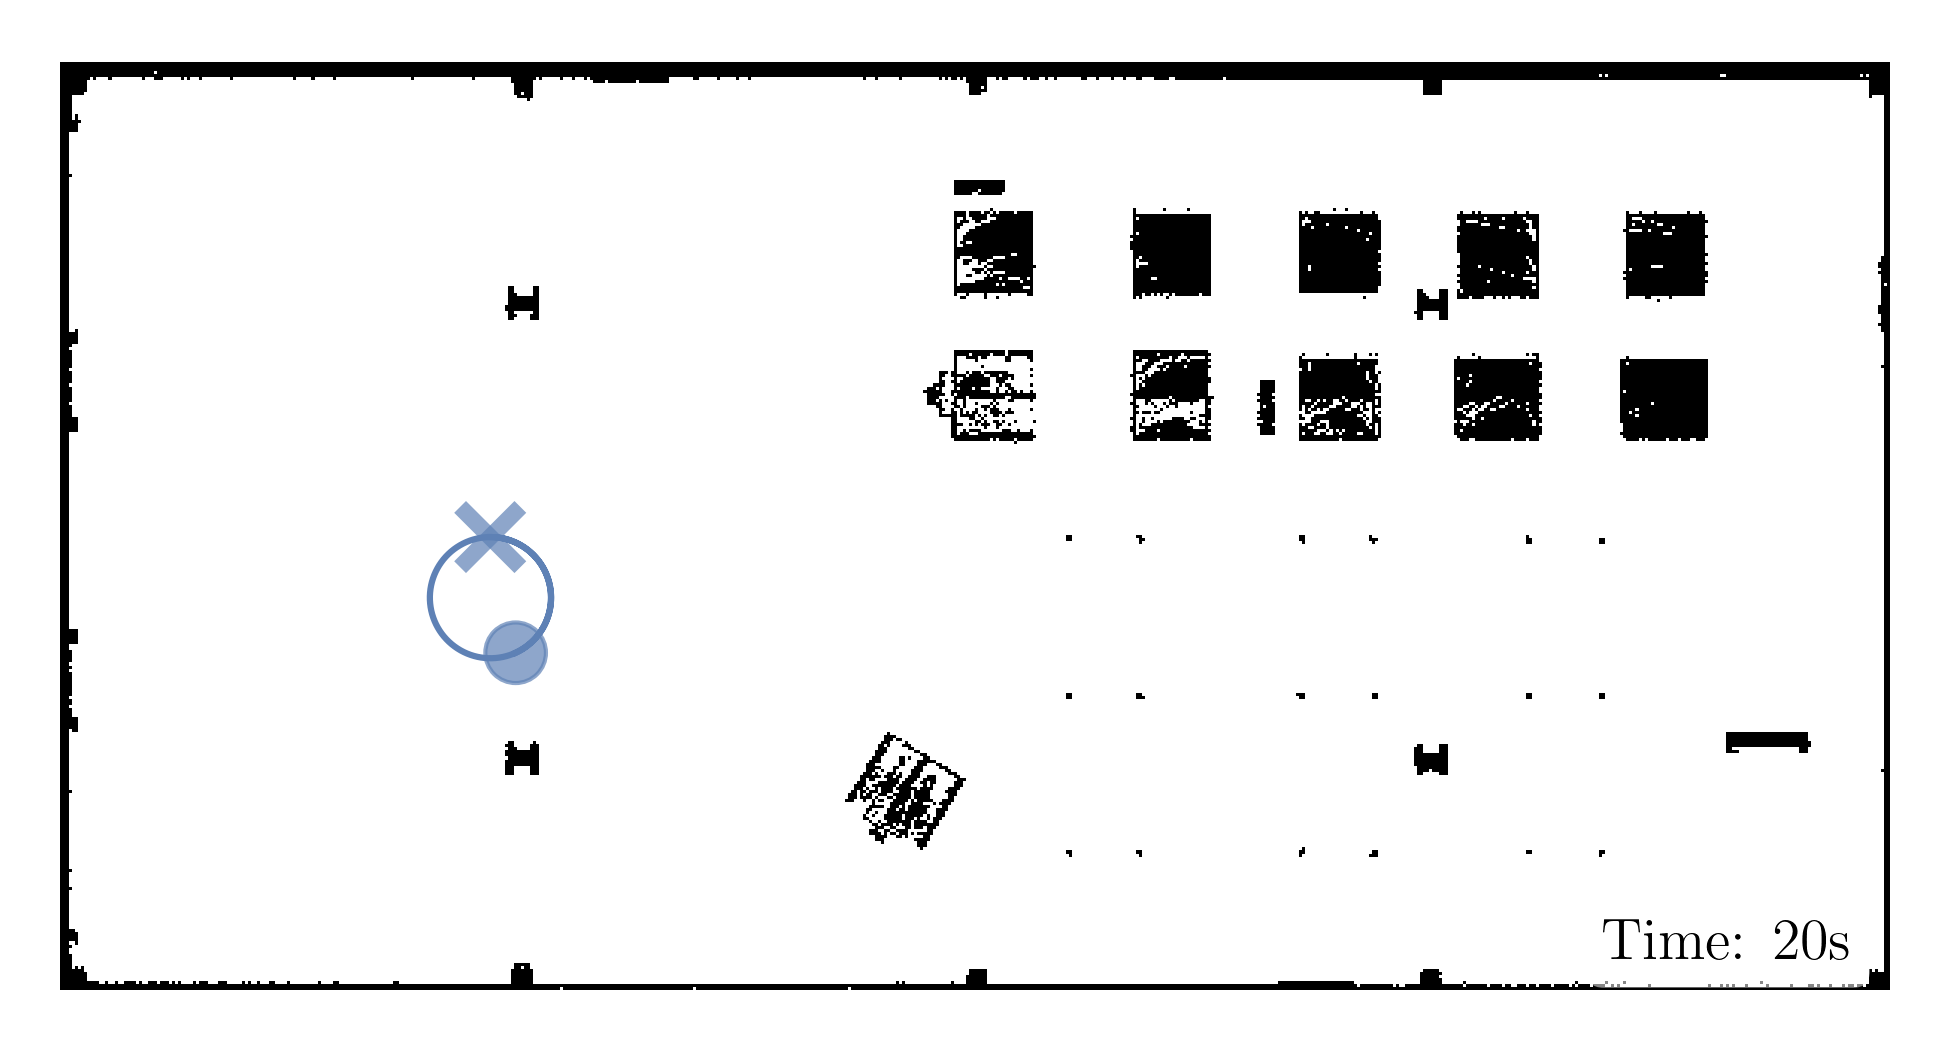
\includegraphics[width=\textwidth]{./figures/plots/consistency/simple-sim-paths-(after-20s).png}
    \caption{Simple Sim}
  \end{subfigure}
  \begin{subfigure}[b]{0.45\textwidth}
    \centering
    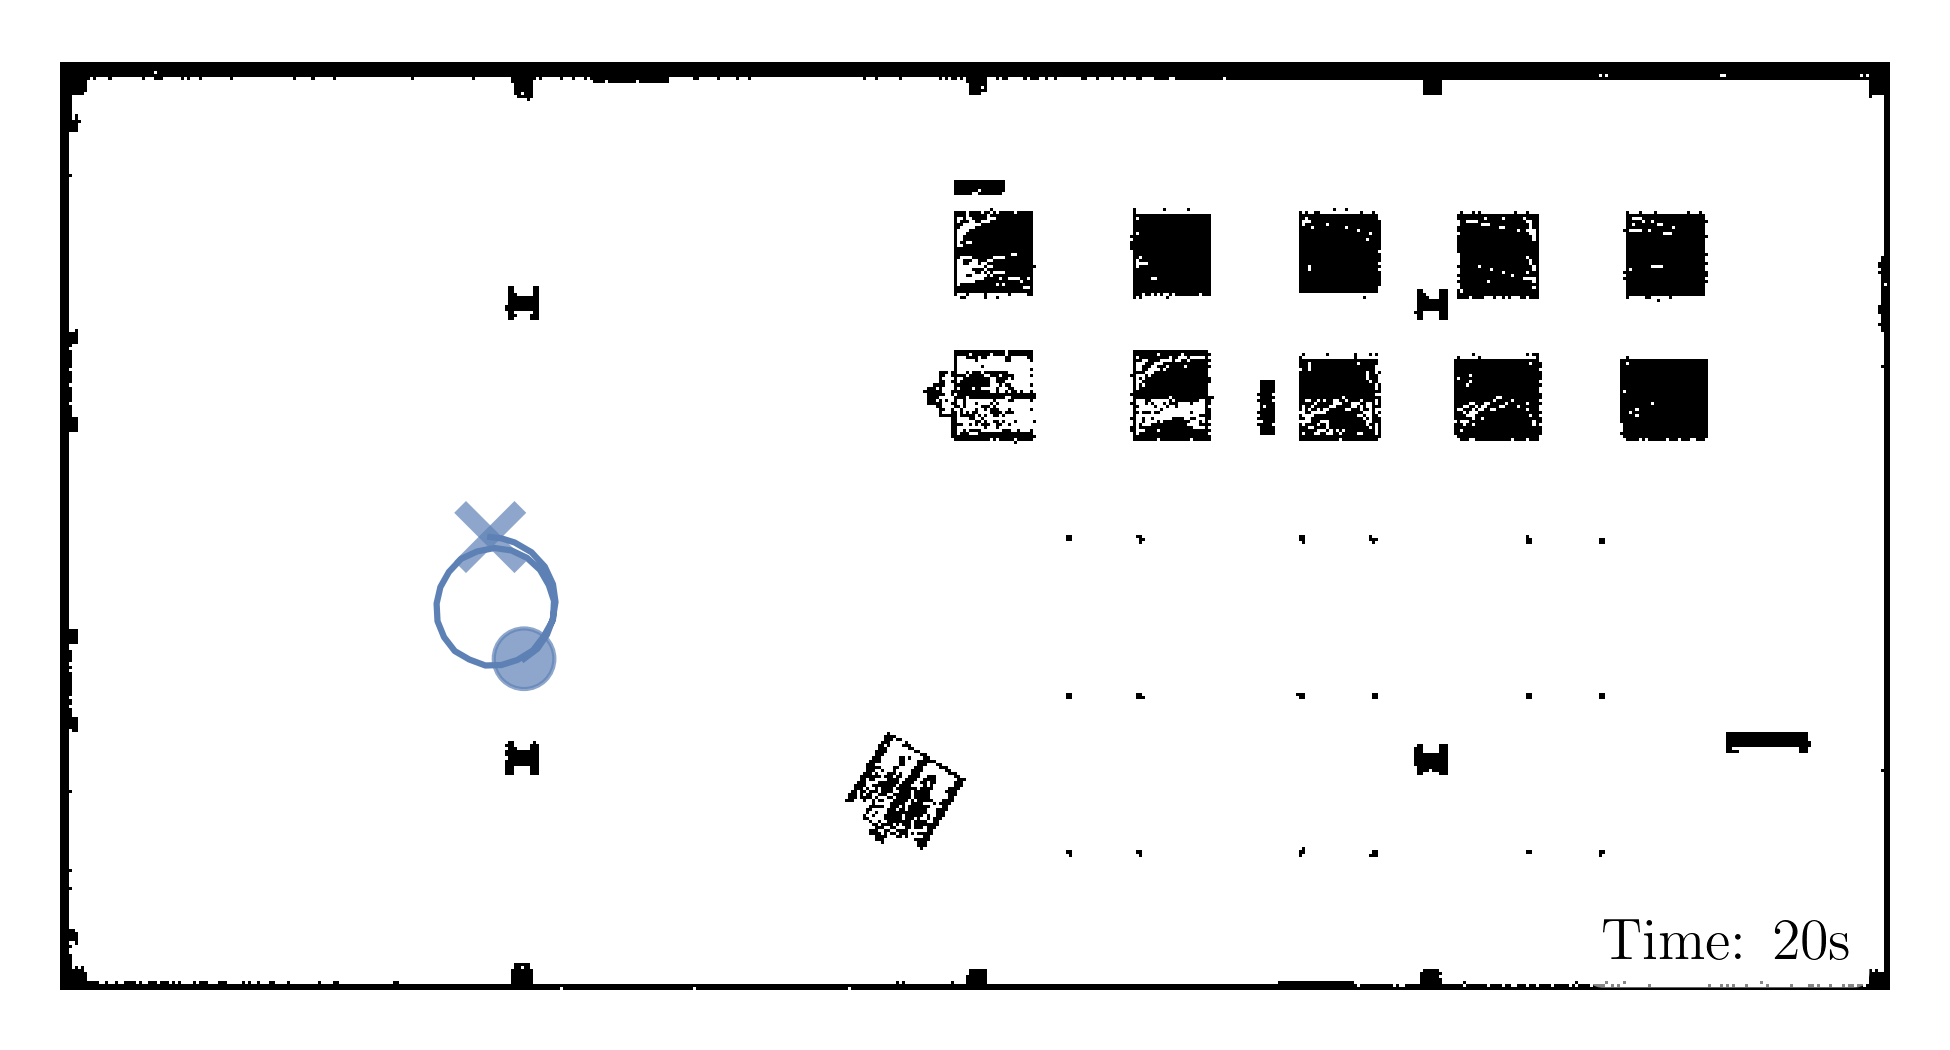
\includegraphics[width=\textwidth]{./figures/plots/consistency/ros-2-paths-(after-20s).png}
    \caption{ROS 2 Gazebo}
  \end{subfigure}
  \caption{Path when running circular behavior in \texttt{simple\_sim} and ROS 2 Gazebo.}
  \label{fig:movement-consistency}
\end{figure}

\subsubsection{Pathing}
A more complex evaluation was performed by comparing search behavior involving dynamic path planning. As shown in \cref{fig:coverage-benchmark}, the coverage curves produced by each simulator are closely aligned, particularly in early and mid-stage exploration. Minor deviations are attributed to non-determinism in Gazebo and slight differences in physics and sensor modeling.

\begin{figure}[H]
  \centering
  \begin{tabular}{cc}
    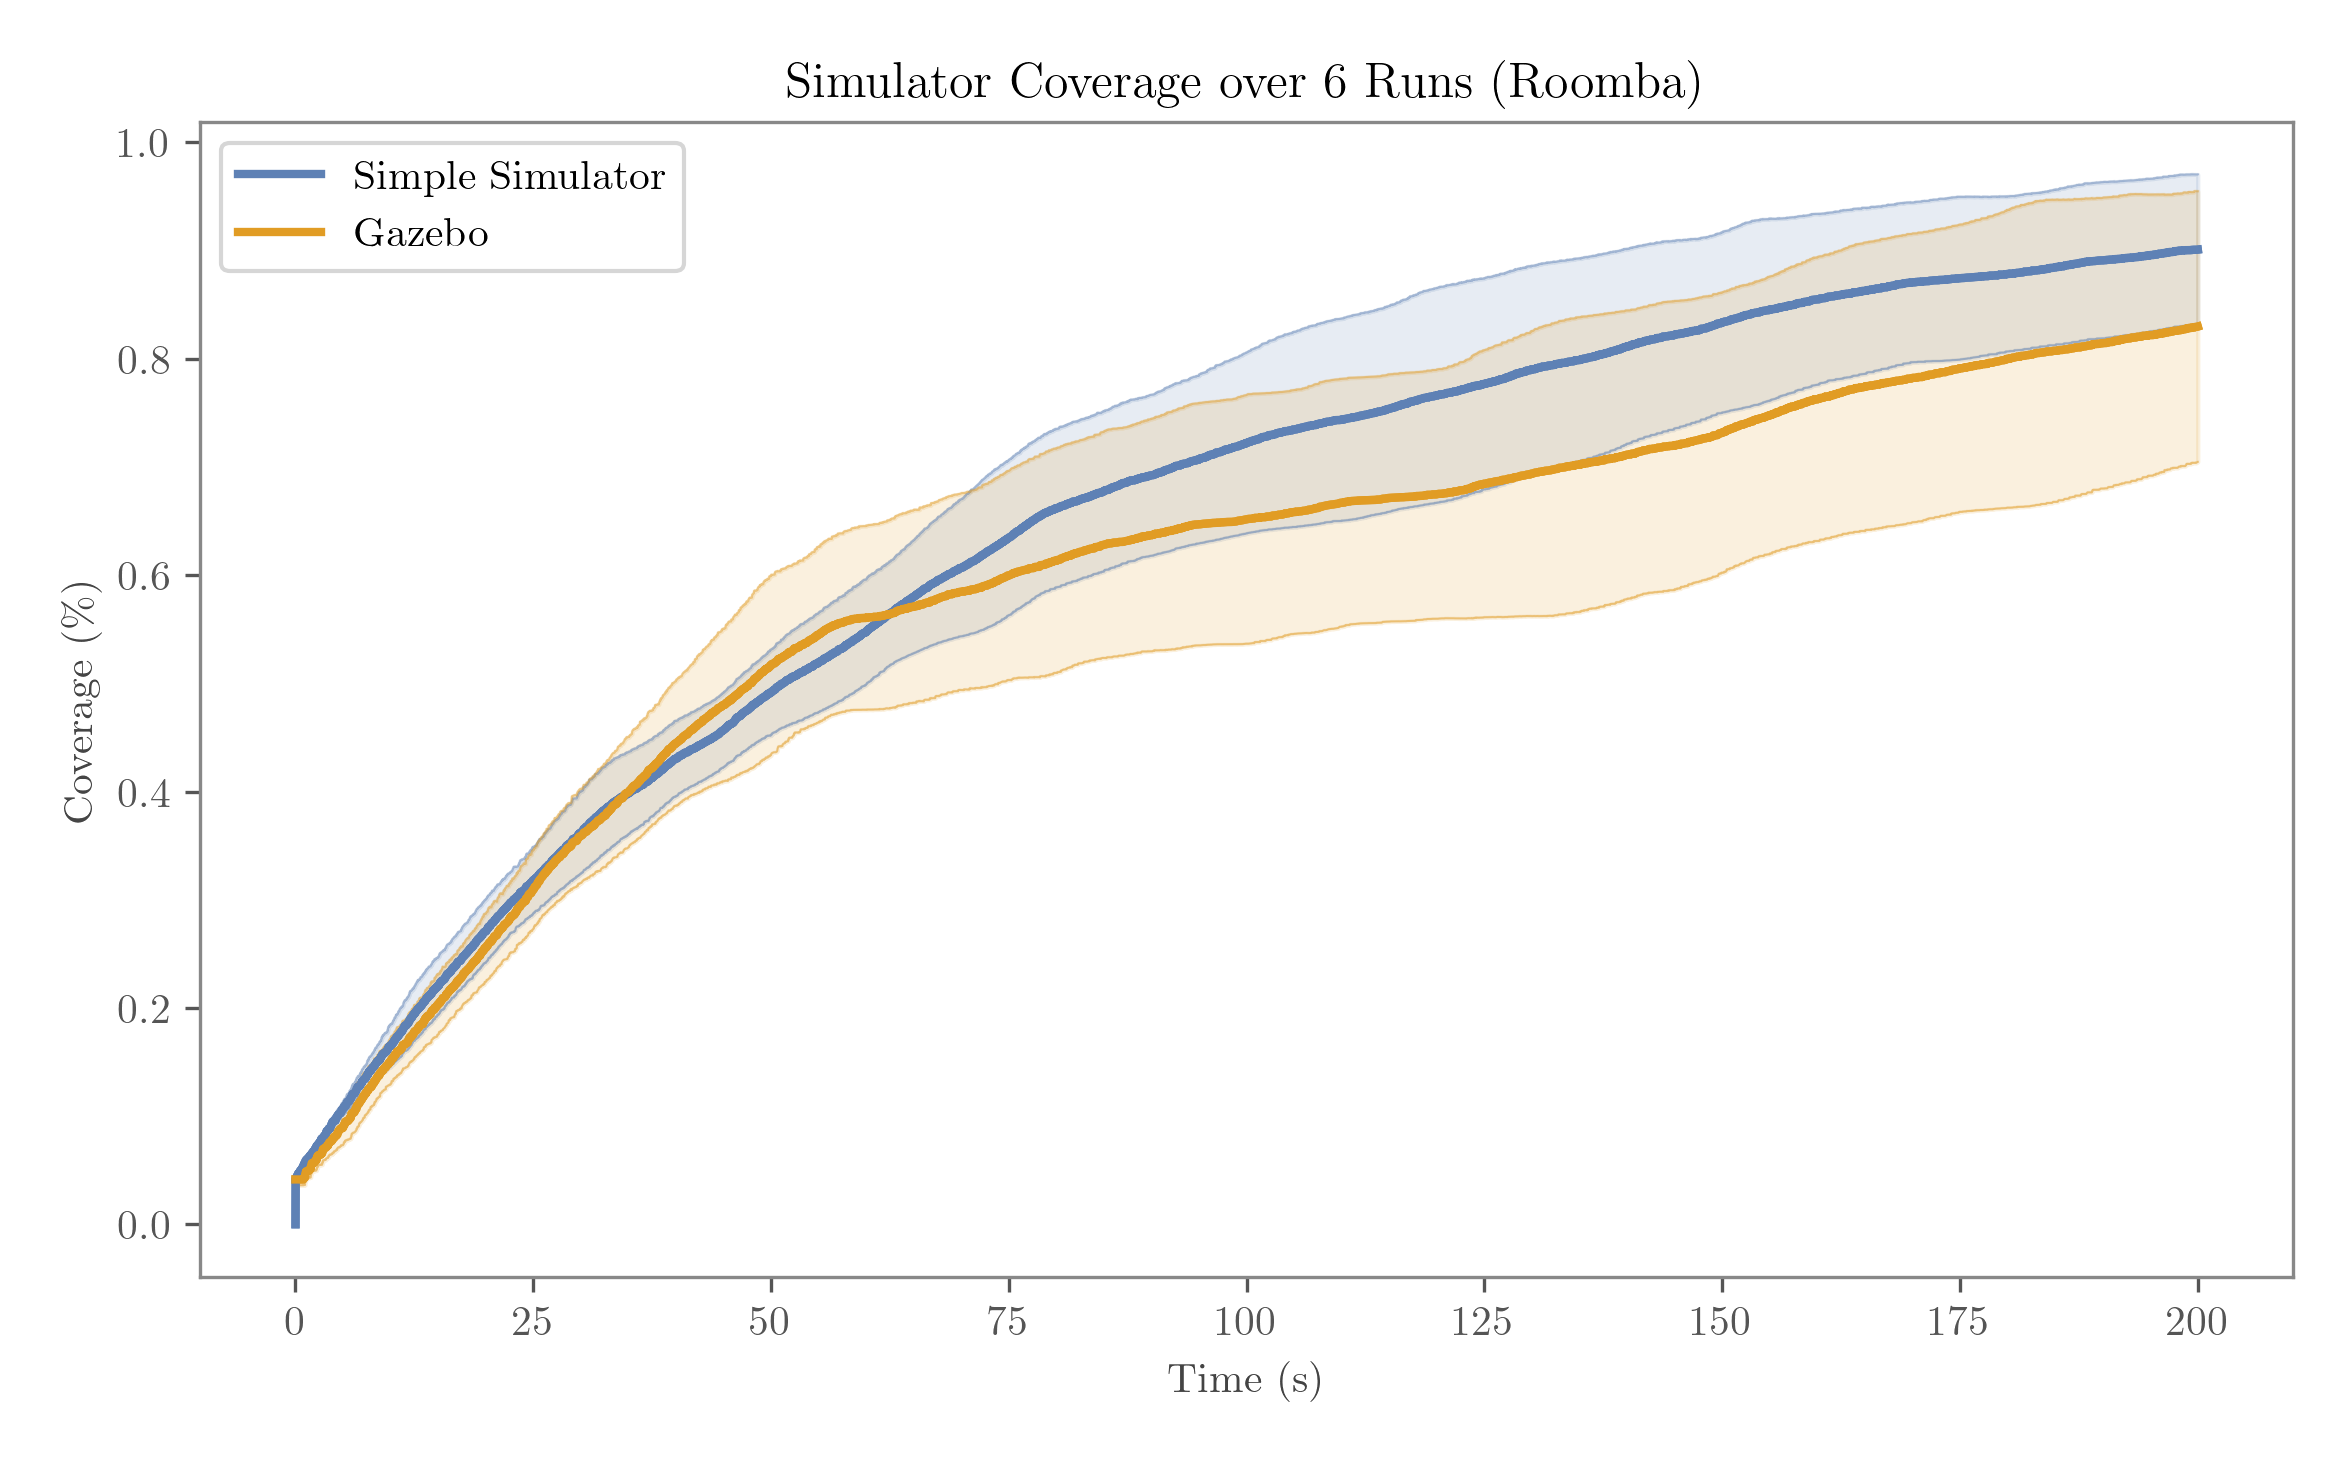
\includegraphics[width=0.45\textwidth]{./figures/plots/consistency/gazebo_vs_simple_sim_roomba.png} &
    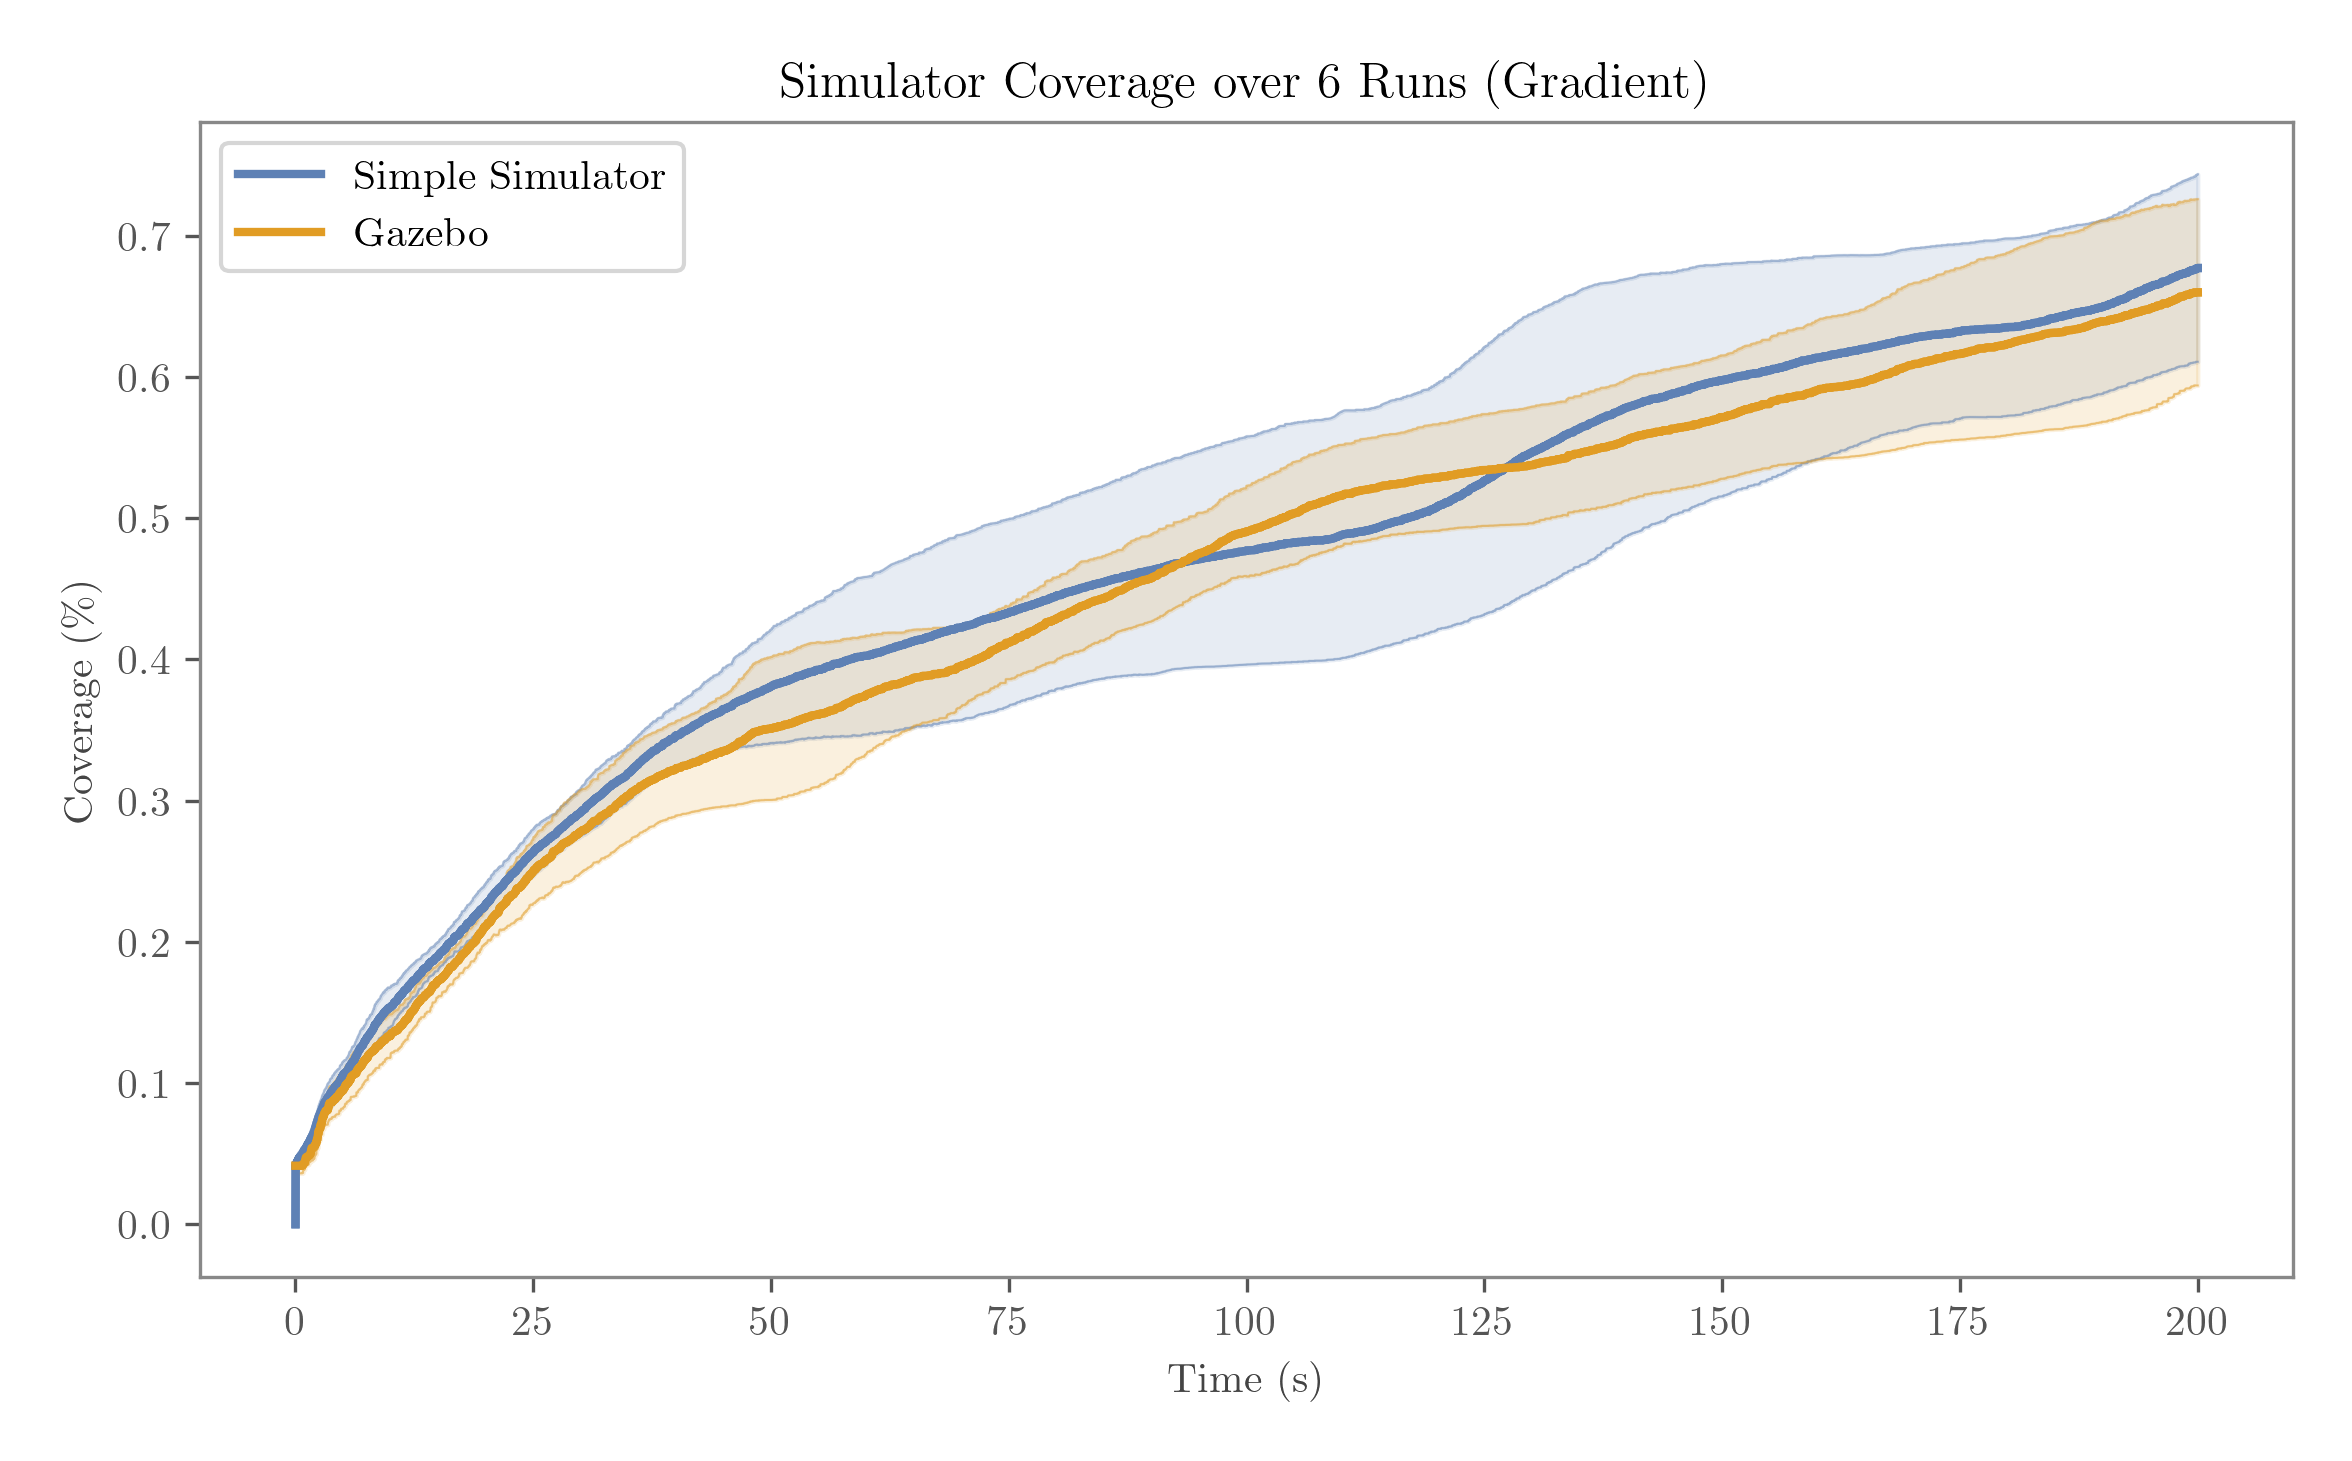
\includegraphics[width=0.45\textwidth]{./figures/plots/consistency/gazebo_vs_simple_sim_gradient.png} \\
    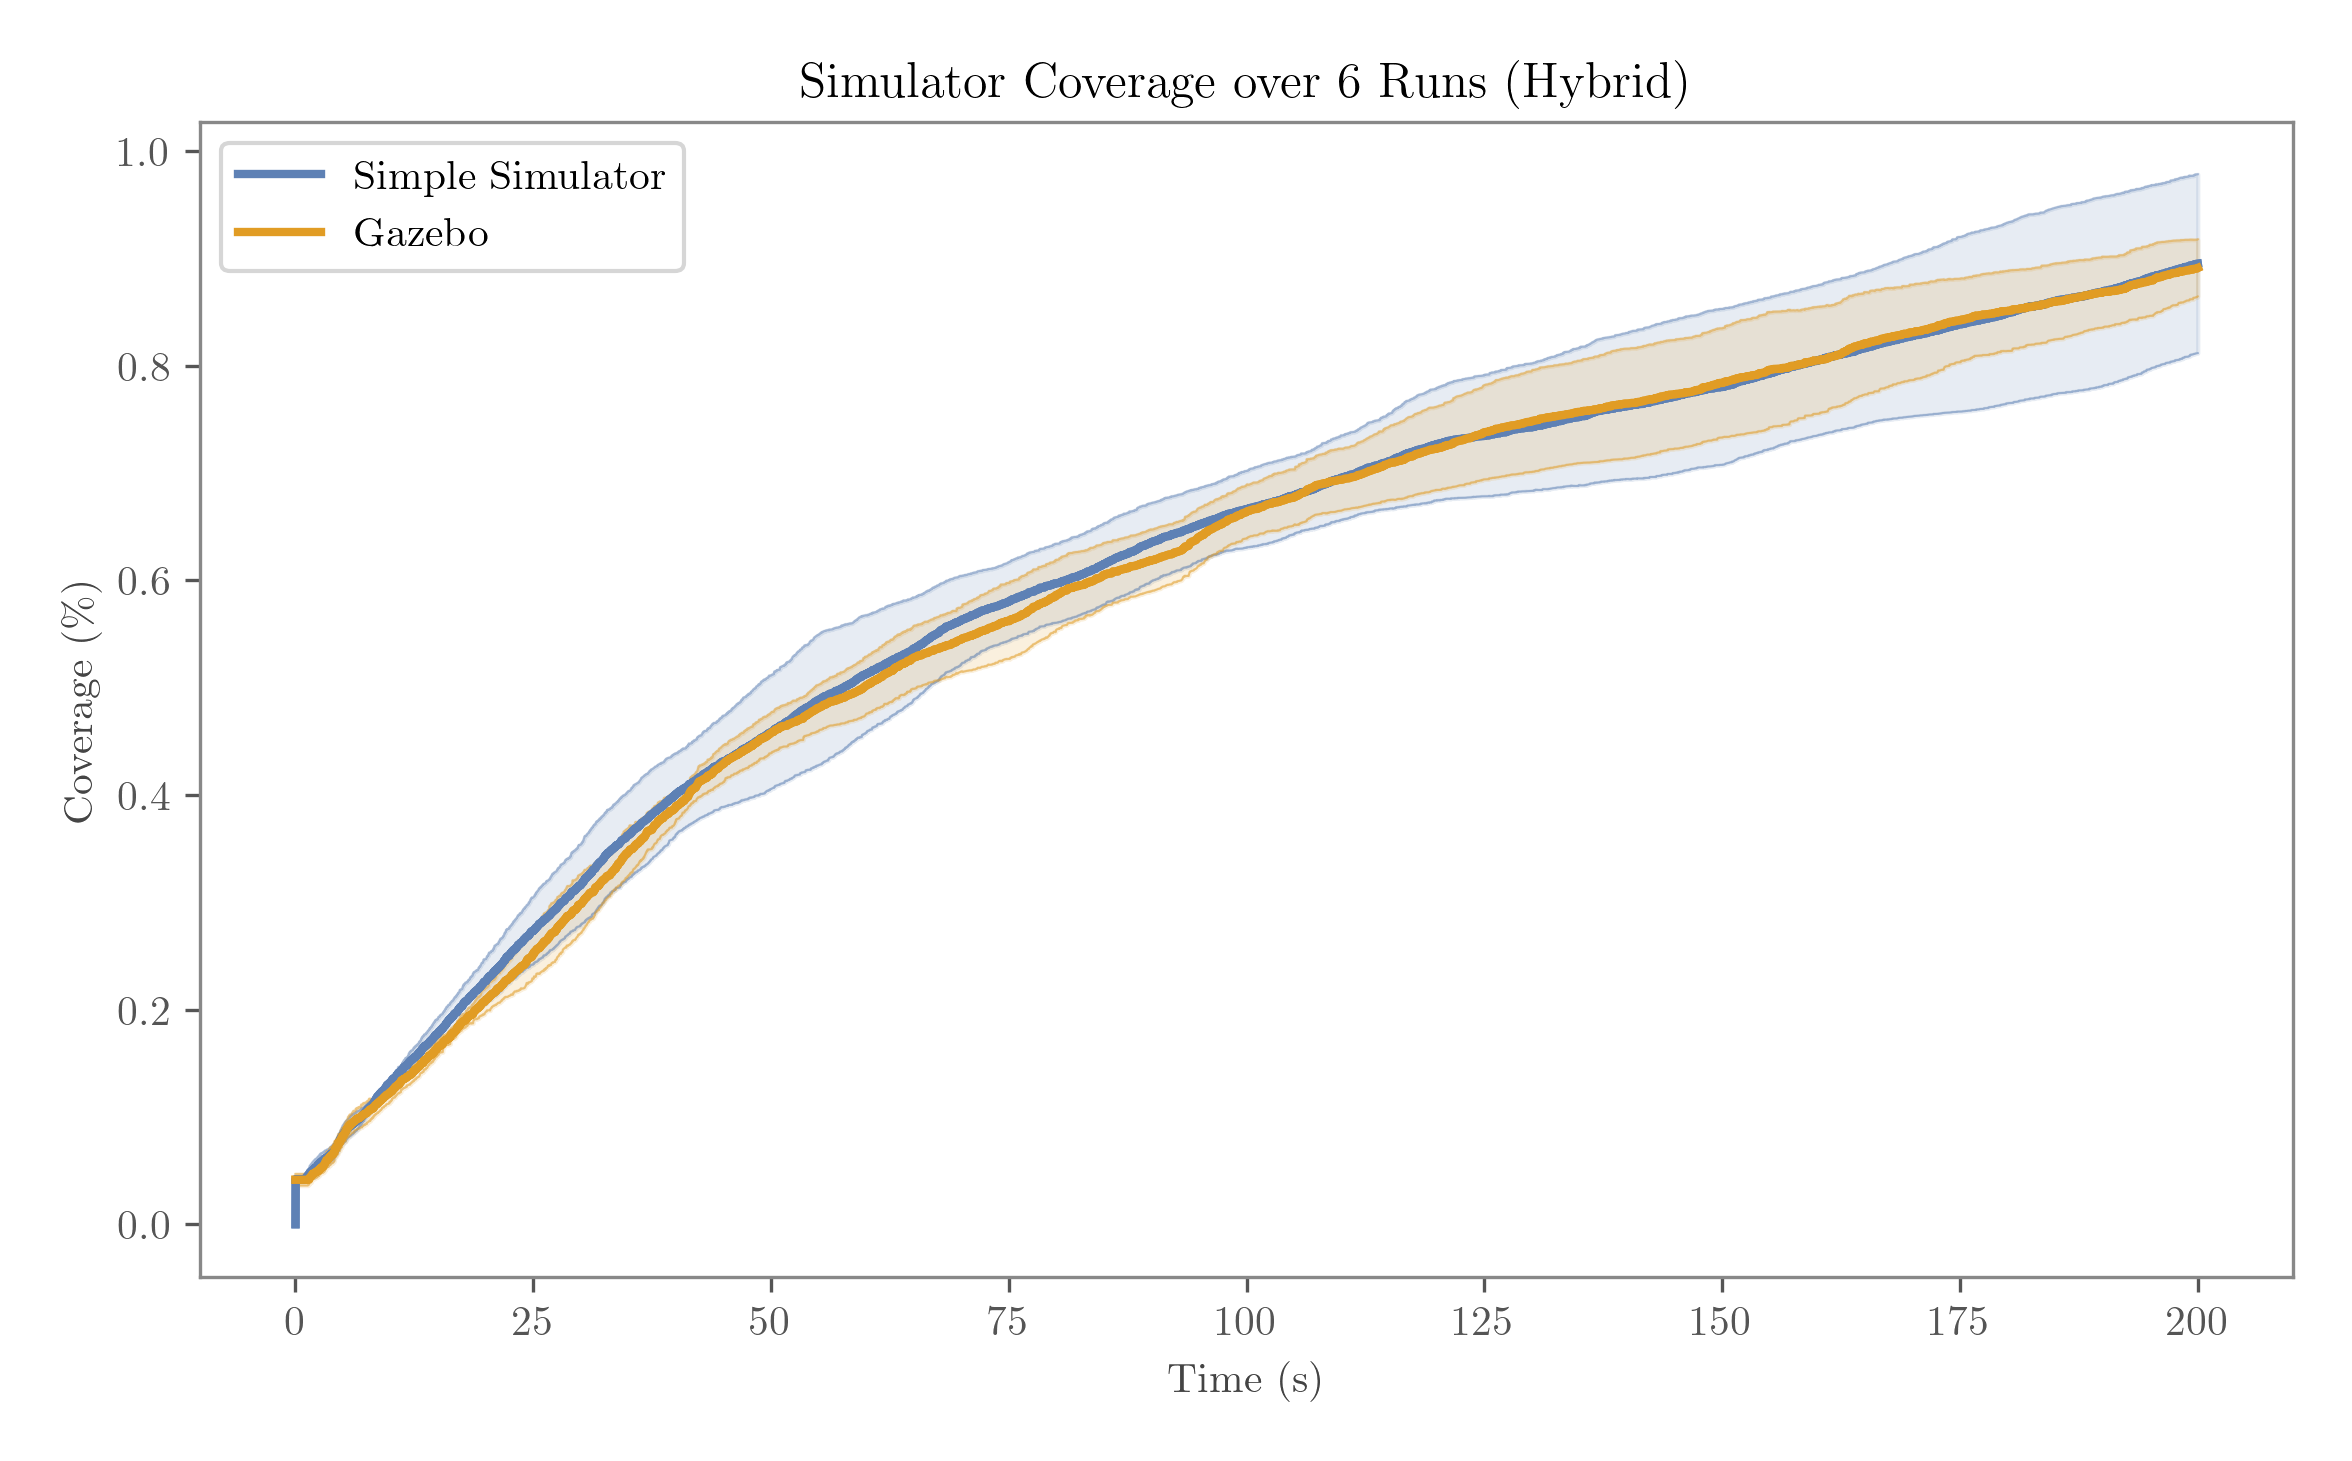
\includegraphics[width=0.45\textwidth]{./figures/plots/consistency/gazebo_vs_simple_sim_hybrid.png} &
    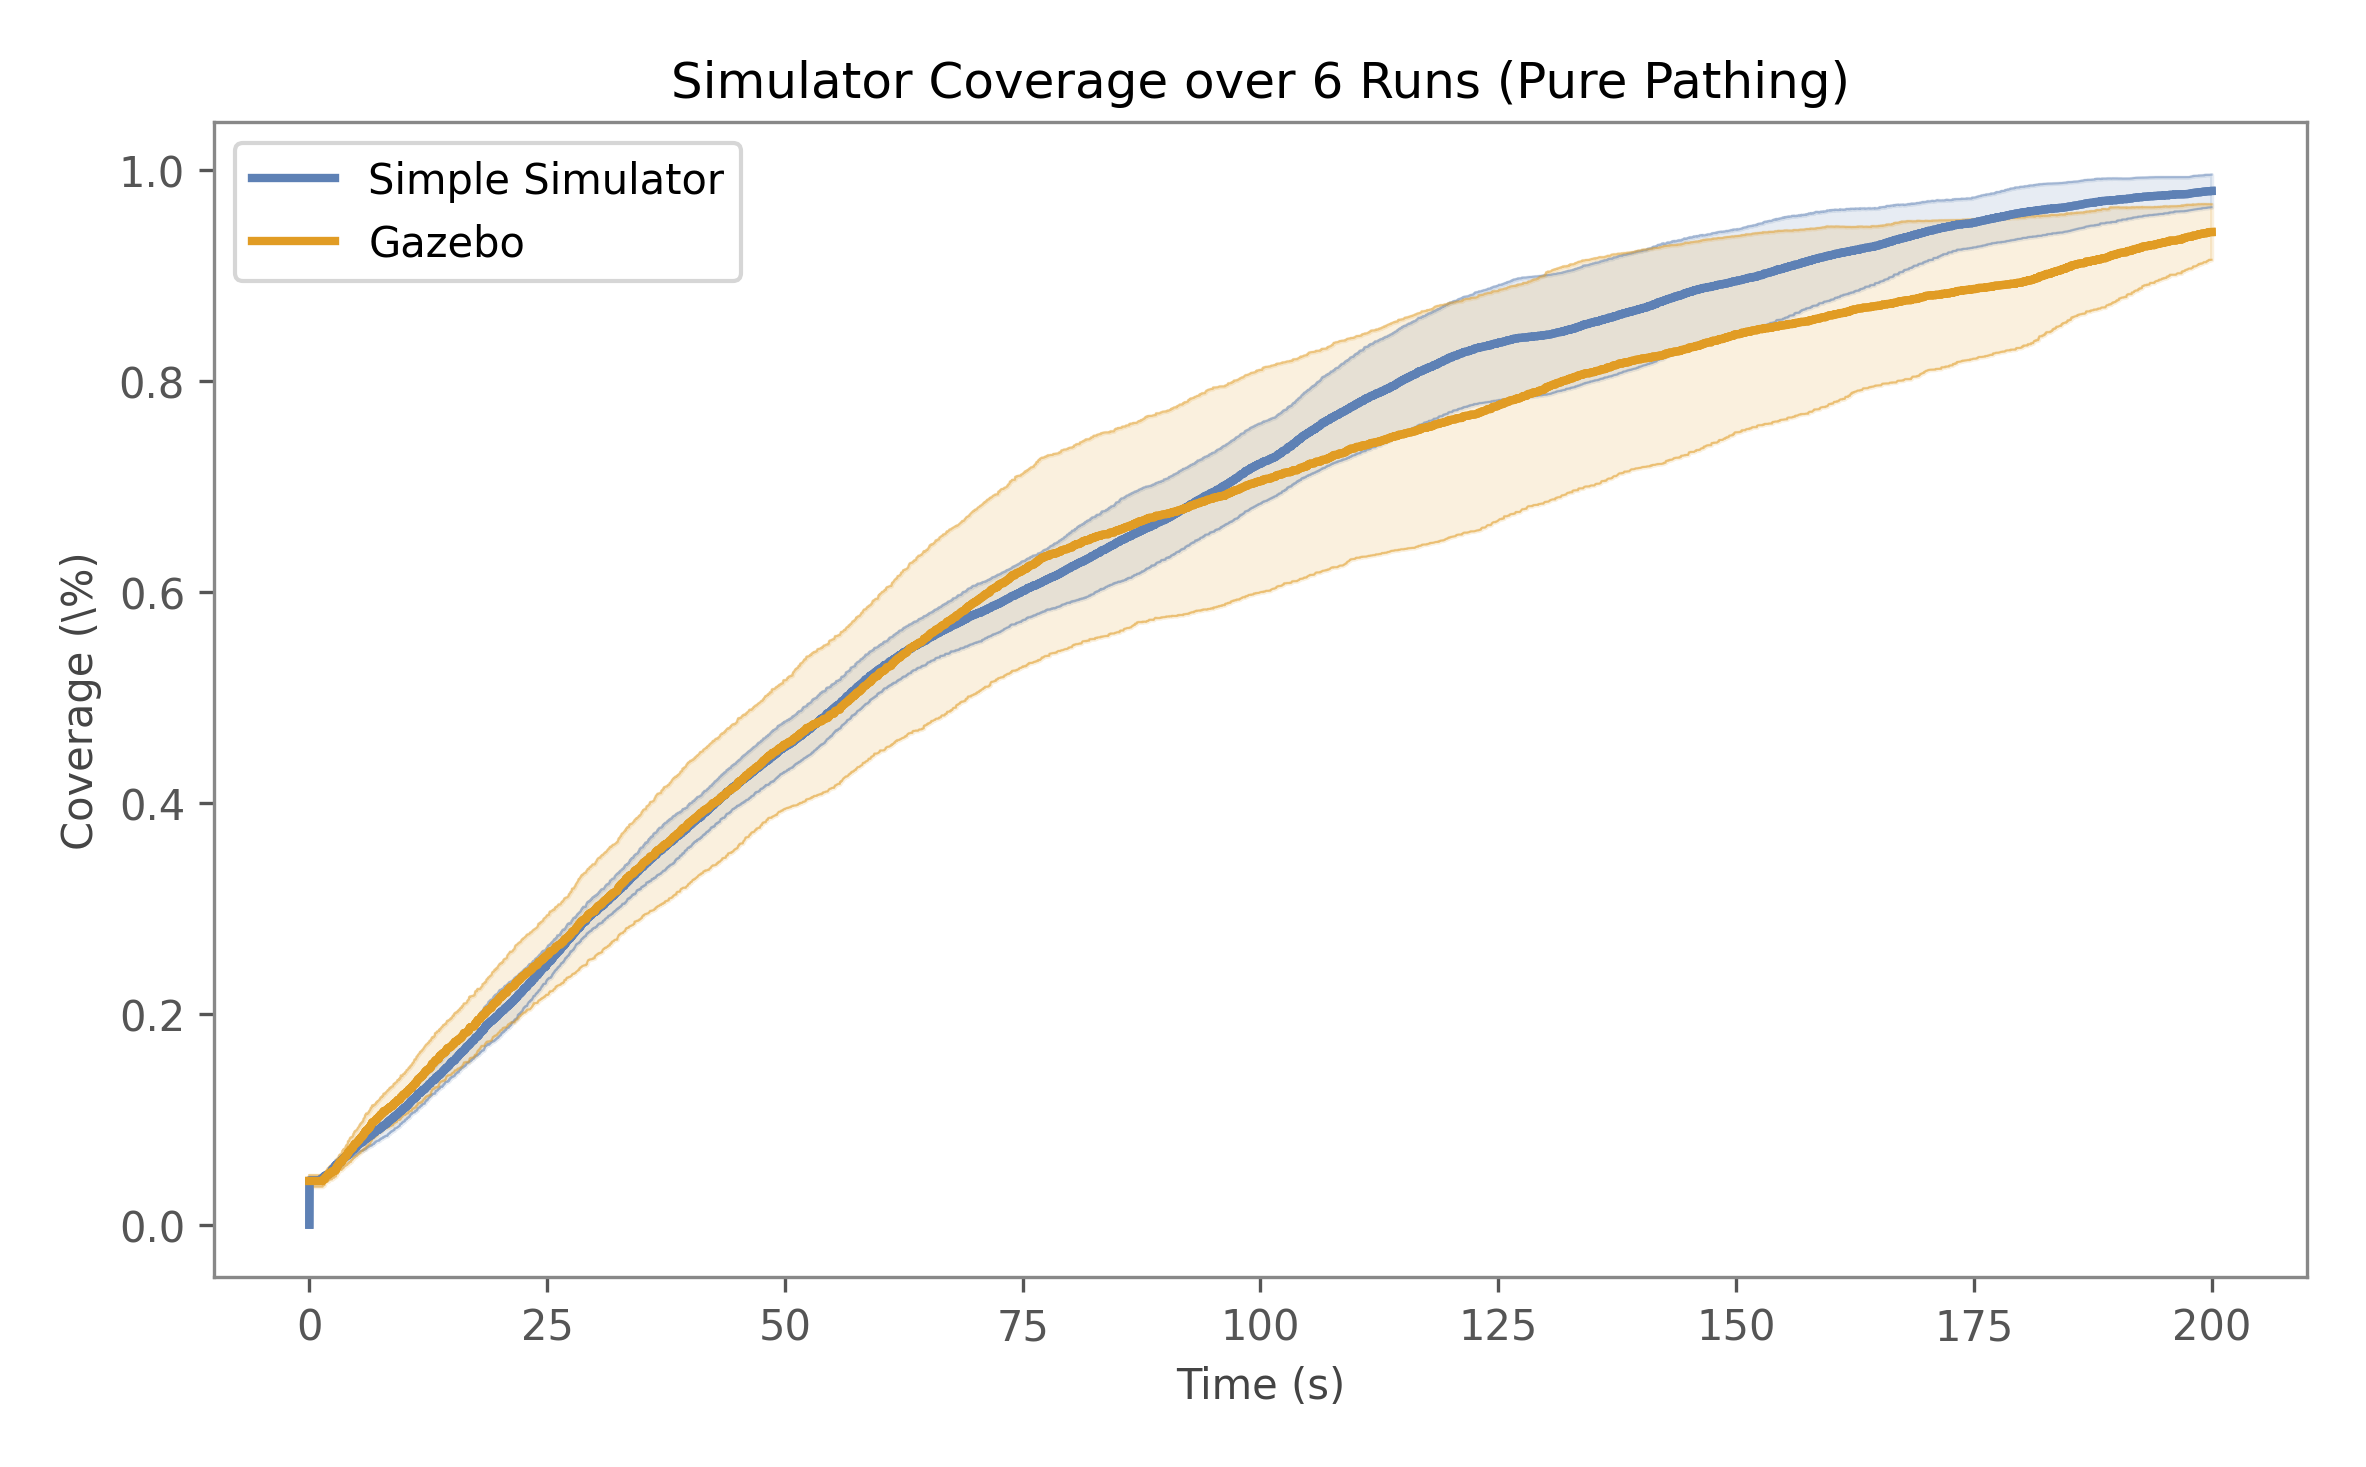
\includegraphics[width=0.45\textwidth]{./figures/plots/consistency/gazebo_vs_simple_sim_pure_pathing.png} \\
  \end{tabular}
  \caption{Comparison of coverage with spread over time between ROS 2 Gazebo and \texttt{simple\_sim}.}
  \label{fig:coverage-benchmark-all}
\end{figure}

\begin{figure}[H]
    \begin{center}
        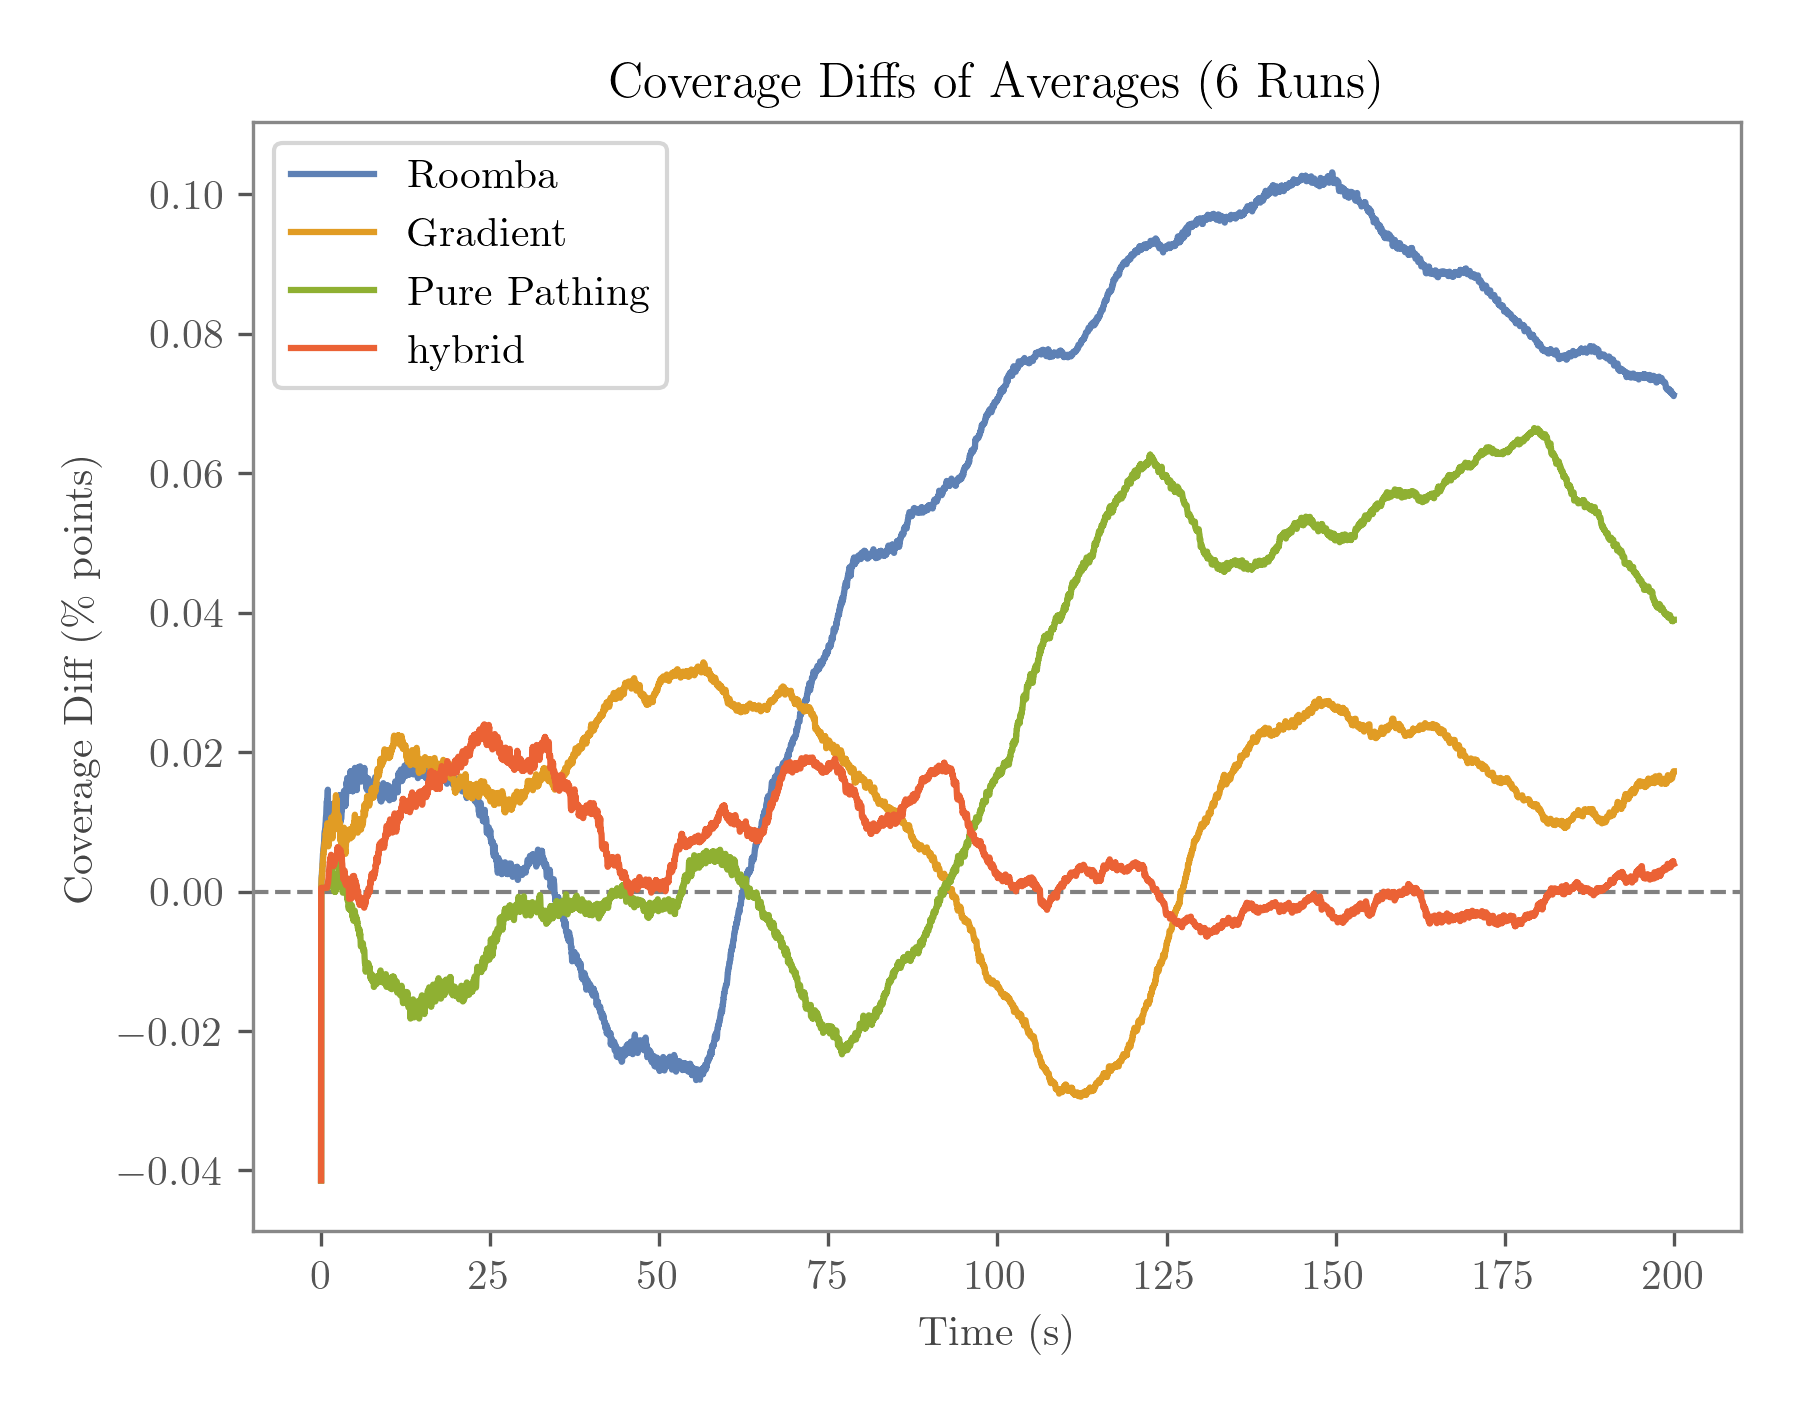
\includegraphics[width=0.95\textwidth]{./figures/plots/consistency/coverage-diffs-of-averages-(6-runs).png}
    \end{center}
    \caption{Comparison of difference in coverage over time between ROS 2 Gazebo and \texttt{simple\_sim}.}
    \label{fig:coverage-benchmark-diff}
\end{figure}

\subsection{Search Algorithm Benchmarks}
To evaluate search efficiency, each algorithm was executed across multiple randomly generated maps. The benchmark shown in \cref{fig:search-coverage-benchmark} presents average coverage over 10 runs, along with minimum and maximum bounds for each time step.

\begin{figure}[H]
    \begin{center}
        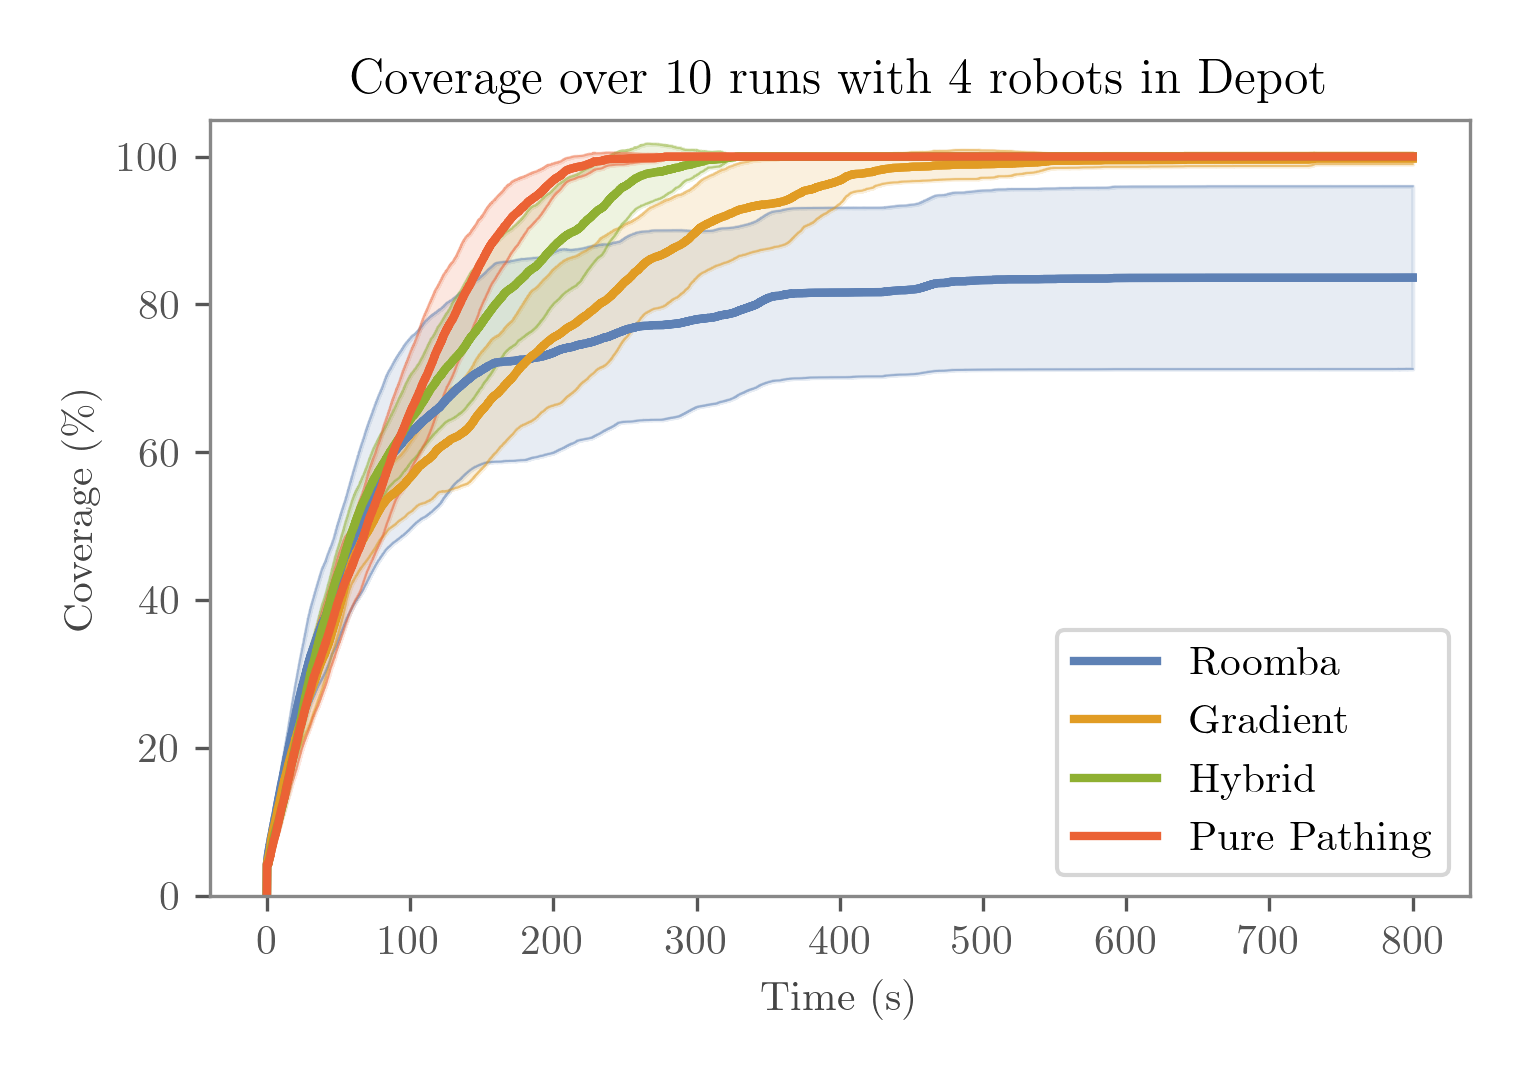
\includegraphics[width=0.95\textwidth]{./figures/plots/benchmarks/coverage-over-10-runs-with-4-robots-in-depot.png}
    \end{center}
    \caption{Coverage performance of search algorithms over 10 runs starting in random positions in the same environment. Shaded regions represent the range between minimum and maximum coverage at each time step.}
    \label{fig:coverage-benchmark}
\end{figure}

All algorithms eventually achieve full coverage, though their exploration efficiency varies significantly. 
Gradient-based methods tend to cover local areas quickly but slow down due to diminishing gradients near fully explored zones. 
Frontier-based methods achieve higher global efficiency by directing robots toward unknown regions, but at a higher computational cost. The hybrid method strikes a balance by switching strategies based on local exploration progress. 
Deep reinforcement learning shows promise but requires further tuning for consistent early-stage performance.

\subsection{Performance}
\subsubsection{Computation Time}
% FIX: Mean line not working
\begin{figure}[H]
    \begin{center}
        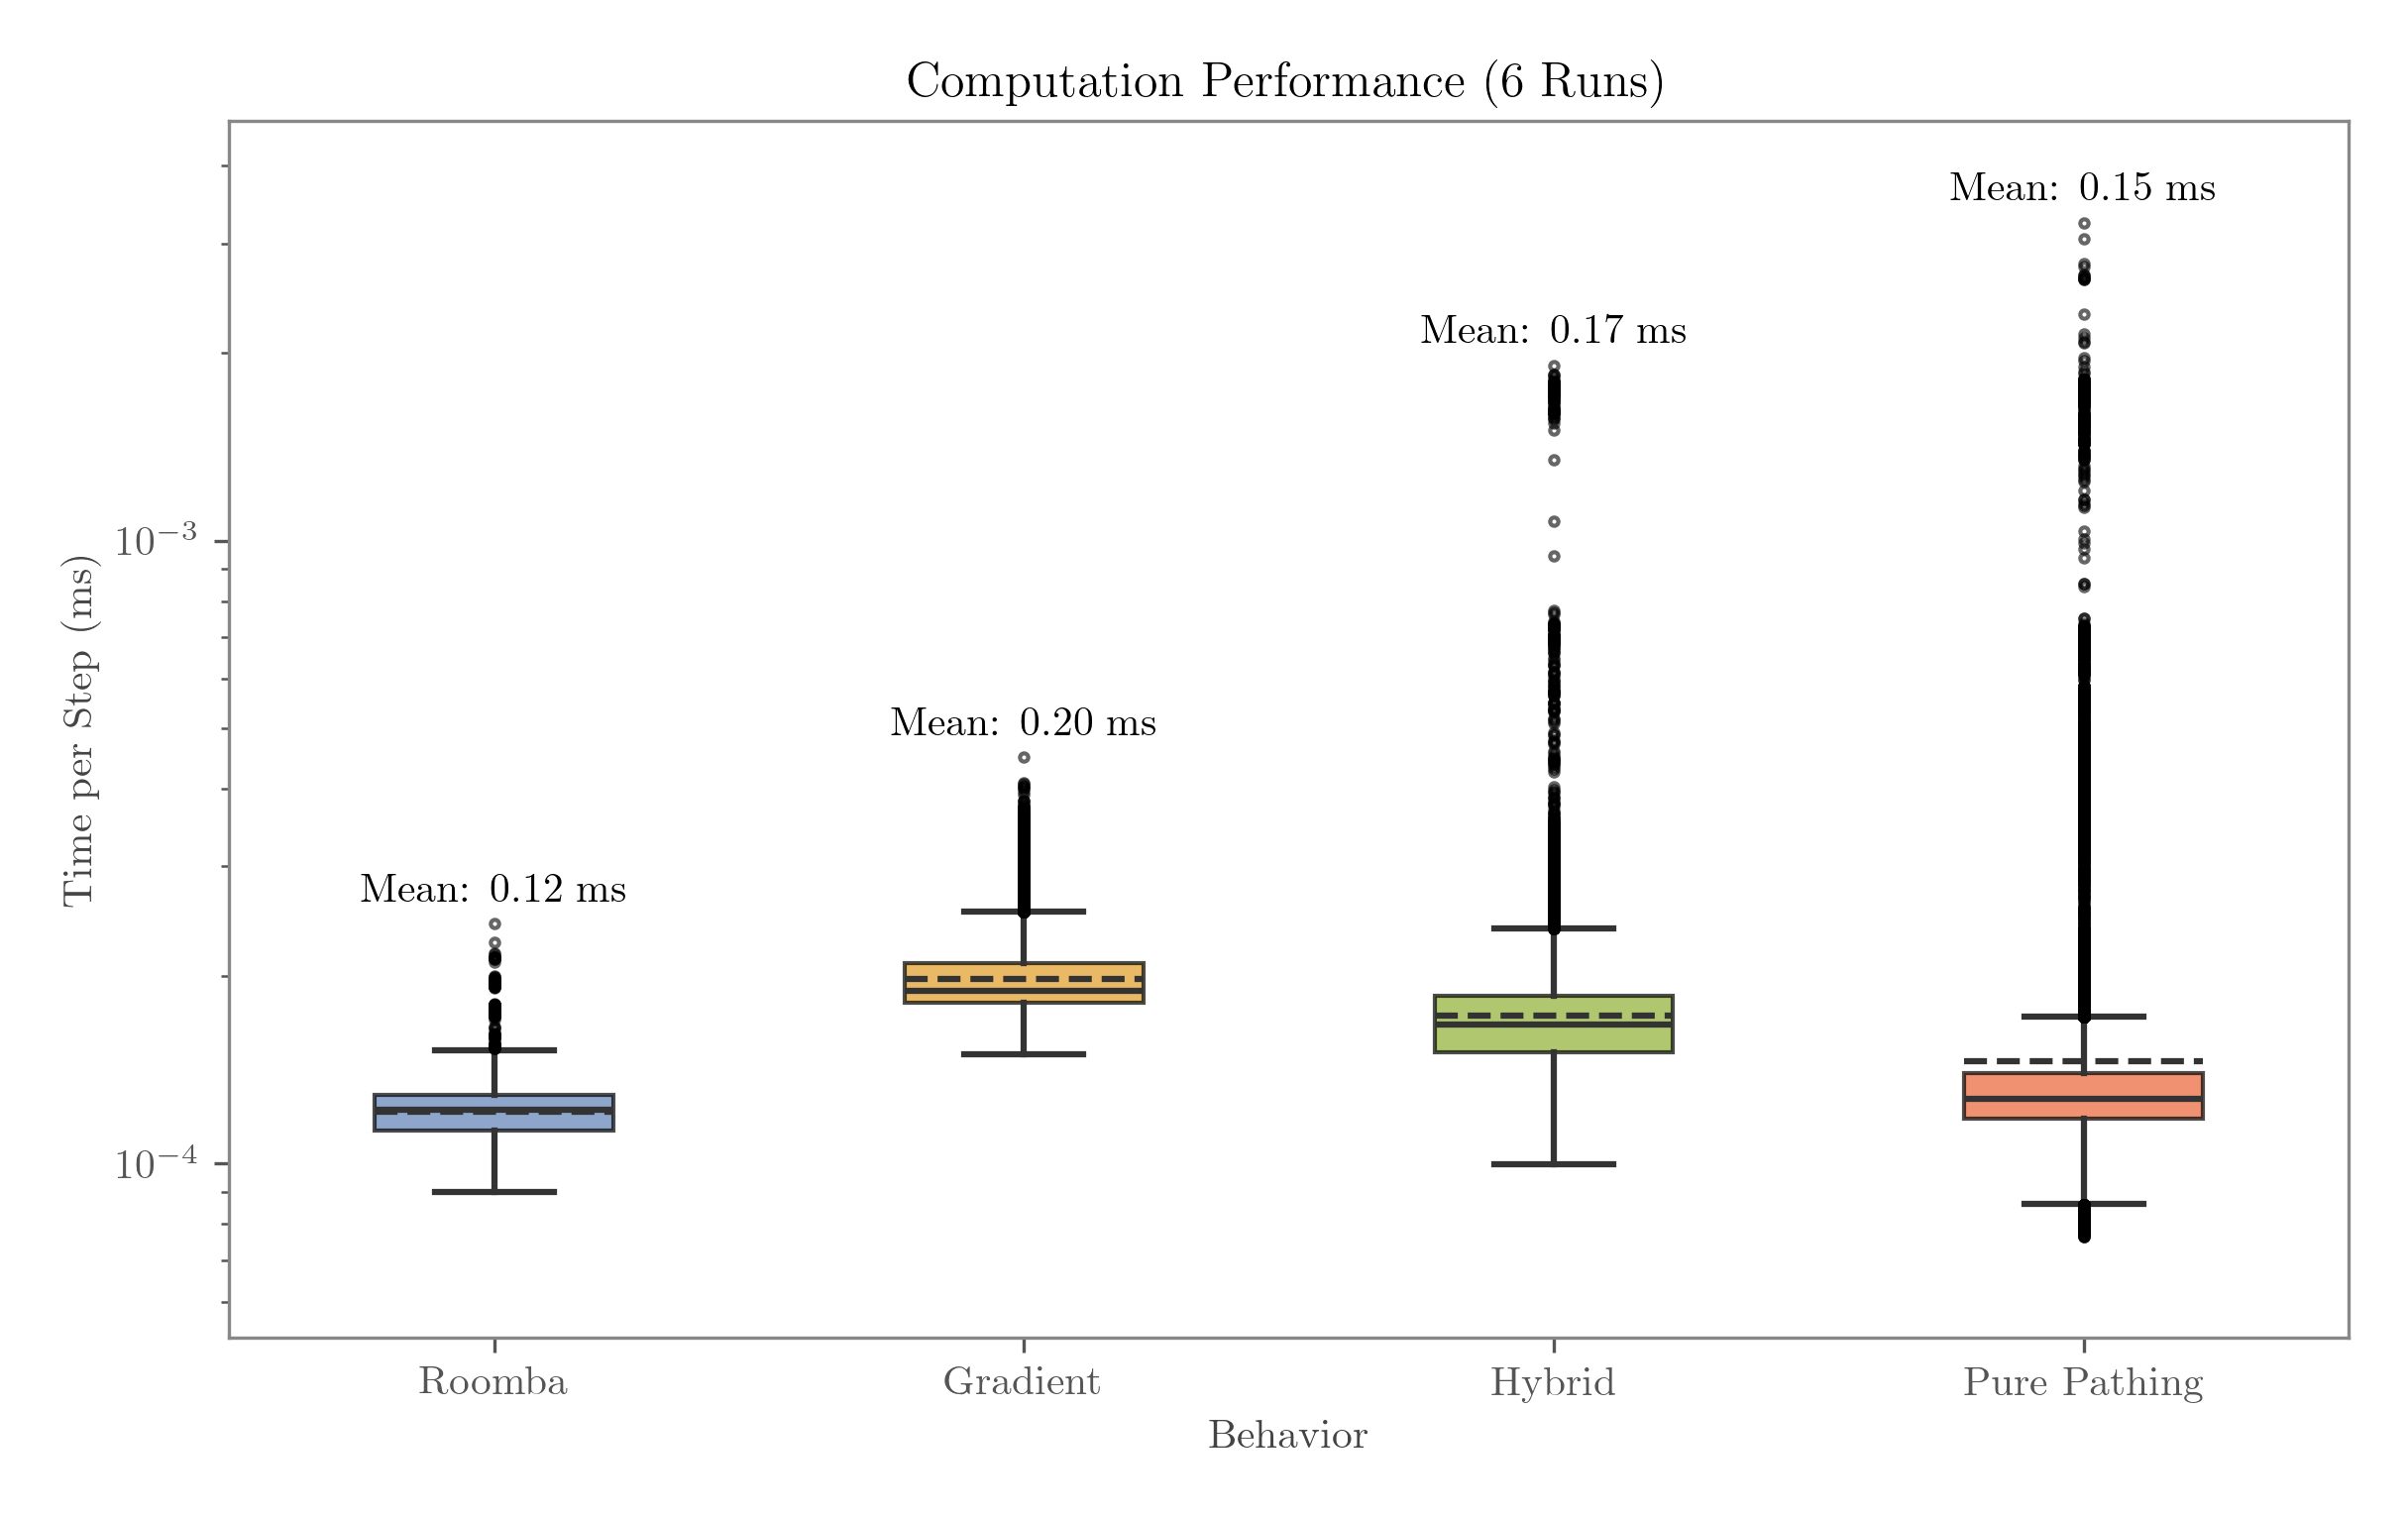
\includegraphics[width=0.95\textwidth]{./figures/plots/computation-performance-(6-runs).png}
    \end{center}
    \caption{Computation time boxplot for each algorithm on the same map.}
    \label{fig:computation-performance}
\end{figure}

\subsubsection{Communication {\color{red}Load}}
\begin{figure}[H]
    \begin{center}
        \includegraphics[width=0.95\textwidth]{./figures/plots/bytes.png}
    \end{center}
    \caption{Message size boxplot for each algorithm on the same map.}
    \label{fig:computation-performance}
\end{figure}
